% !TEX program = xelatex
\documentclass[9pt, aspectratio=169]{beamer}
\usetheme{metropolis}
\usefonttheme{professionalfonts}

% --- Modern Font Setup ---
\usepackage[T1]{fontenc}
\usepackage{FiraSans}  % Modern, elegant sans-serif font family
\usepackage[scaled=0.95]{FiraMono}  % Matching monospace font

% Lighter, more refined font weights
\renewcommand{\seriesdefault}{l}  % Light weight as default
\renewcommand{\bfseries}{\fontseries{sb}\selectfont}  % Semi-bold instead of bold

% Custom font sizing - more refined
\setbeamerfont{title}{size=\Large, series=\fontseries{m}\selectfont}
\setbeamerfont{subtitle}{size=\normalsize, series=\fontseries{l}\selectfont}
\setbeamerfont{author}{size=\small, series=\fontseries{l}\selectfont}
\setbeamerfont{date}{size=\small, series=\fontseries{l}\selectfont}
\setbeamerfont{frametitle}{size=\normalsize, series=\fontseries{m}\selectfont}
\setbeamerfont{framesubtitle}{size=\footnotesize, series=\fontseries{l}\selectfont}
\setbeamerfont{block title}{size=\normalsize, series=\fontseries{m}\selectfont}
\setbeamerfont{block body}{size=\small}
\setbeamerfont{itemize/enumerate body}{size=\small}
\setbeamerfont{itemize/enumerate subbody}{size=\footnotesize}
\setbeamerfont{section in toc}{size=\normalsize, series=\fontseries{m}\selectfont}
\setbeamerfont{section title}{size=\Large, series=\fontseries{m}\selectfont}

% --- Color Definitions ---
% Primary Theme Colors
\definecolor{PrimaryColor}{RGB}{33,52,72}         % Deep navy
\definecolor{SecondaryColor}{RGB}{84,119,146}     % Desaturated blue-gray
\definecolor{AccentColor}{RGB}{100,156,165}       % Soft steel blue
\definecolor{black}{RGB}{0,0,0}
\definecolor{BackgroundColor}{RGB}{245,247,250}   % Very light cool gray/blue-tinted white
\definecolor{TextColor}{RGB}{40,55,70}            % Darker, cool-toned charcoal
\definecolor{LightGray}{RGB}{220,225,230}         % Soft, cool light gray
\definecolor{DarkGray}{RGB}{70,90,105}            % Cool-toned dark gray

% --- Theme Customization ---
\setbeamercolor{background canvas}{bg=BackgroundColor}
\setbeamercolor{normal text}{fg=TextColor}
\setbeamercolor{frametitle}{bg=PrimaryColor, fg=white}
\setbeamercolor{section in toc}{fg=PrimaryColor}
\setbeamercolor{block title}{bg=PrimaryColor!80, fg=white}
\setbeamercolor{block body}{bg=PrimaryColor!10}
\setbeamercolor{alerted text}{fg=AccentColor}
\setbeamercolor{itemize item}{fg=PrimaryColor}
\setbeamercolor{itemize subitem}{fg=SecondaryColor}

% Progress bar
\setbeamercolor{progress bar}{fg=AccentColor, bg=LightGray}

% --- Packages ---
\usepackage[utf8]{inputenc}
\usepackage{url}
\usepackage{booktabs}
\usepackage{amsmath, amssymb, amsfonts}
\usepackage{fontawesome5}
\usepackage{pifont}
\usepackage[most]{tcolorbox}
\tcbuselibrary{skins, listings}
\usepackage{colortbl}
\usepackage{array}
\usepackage{adjustbox}
\usepackage{ragged2e}

% --- Packages for plotting discrete and continuous signals and spectrums ---
\usepackage{tikz}
\usepackage{circuitikz} % Useful for signal processing block diagrams
\usepackage{pgfplots}
\usepackage{graphicx}
\usepackage{caption}
\usepackage{subcaption}

\usetikzlibrary{shapes.callouts, positioning, arrows.meta, shapes.geometric, shadows, calc, patterns, backgrounds, shadings, fit, chains, decorations.pathreplacing, intersections}
\usepgfplotslibrary{fillbetween}
\usepgfplotslibrary{polar}
\pgfplotsset{compat=1.18}
\pgfplotsset{
    plot coordinates/math parser=false,
    signal/.style={thick, color=PrimaryColor},
    spectrum/.style={thick, color=AccentColor},
    discrete/.style={ycomb, mark=*, mark options={fill=white, draw=PrimaryColor}, color=PrimaryColor, thick},
}

% --- Custom Commands ---
\newcommand{\cmark}{\textcolor{PrimaryColor}{\ding{51}}}
\newcommand{\xmark}{\textcolor{AccentColor}{\ding{55}}}
\newcommand{\highlight}[1]{\textcolor{PrimaryColor}{\textbf{#1}}}

% --- Custom tcolorbox environments ---
\newtcolorbox{conceptbox}[1]{
    colback=PrimaryColor!10,
    colframe=PrimaryColor,
    title=#1,
    fonttitle=\small\bfseries,
    fontupper=\small,
    rounded corners
}

\newtcolorbox{insightbox}[1]{
    colback=AccentColor!10,
    colframe=AccentColor,
    title=#1,
    fonttitle=\small\bfseries,
    fontupper=\small,
    rounded corners
}

\newtcolorbox{algorithmbox}[1]{
    colback=SecondaryColor!10,
    colframe=SecondaryColor,
    title=#1,
    fonttitle=\small\bfseries,
    fontupper=\small,
    rounded corners
}

\newtcblisting{codelistingbox}[2][]{
    colback=SecondaryColor!10,
    colframe=SecondaryColor,
    title=#2,
    fonttitle=\small\bfseries,
    rounded corners,
    listing only,
    listing options={
            language=#1,
            basicstyle=\ttfamily\footnotesize,
            keywordstyle=\color{PrimaryColor}\bfseries,
            commentstyle=\color{SecondaryColor}\itshape,
            stringstyle=\color{AccentColor},
            numbers=left,
            numberstyle=\tiny\color{DarkGray},
            stepnumber=1,
            showstringspaces=false,
            tabsize=4
        }
}


\subtitle{Signals and Linear Systems}
\date{}
\author{Ashrafur Rahman\\Lecturer, CSE, BUET}
\institute{ashrafur@cse.buet.ac.bd}


\title{Advanced FFT Algorithms and Applications}

\begin{document}

\maketitle

\begin{frame}{Outline}
    \begin{itemize}
        \item \textbf{Advanced FFT Algorithms}
              \begin{itemize}
                  \item Radix-2 \& Radix-3 DIT Tabular Interpretation
                  \item General Cooley-Tukey Matrix Formulation
              \end{itemize}
        \item \textbf{Applications of FFT:} Fast Convolution
              \begin{itemize}
                  \item Circular Convolution
                  \item Linear Convolution via Zero-Padding
                        %   \item Fast Convolution Complexity
              \end{itemize}
              % \item \textbf{FFT for Prime $N$:} Bluestein's Algorithm
              %       \begin{itemize}
              %           \item Chirp-Z Transform Derivation
              %           \item Bluestein's Convolution Interpretation
              %       \end{itemize}
    \end{itemize}
\end{frame}

\section{Advanced Matrix Interpretations of FFT}

\begin{frame}{Revisiting Radix-2: A Tabular View}
    \begin{itemize}
        \item Previously, we derived Radix-2 DIT purely algebraically.
        \item We divided the input into even and odd indices and calculated their DFTs $G[k]$ and $H[k]$.
        \item Then we combined them using the butterfly operation:
              \begin{align*}
                  X[k]     & = G[k] + W_N^k H[k] \\
                  X[k+N/2] & = G[k] - W_N^k H[k]
              \end{align*}
        \item We can think about this in a different, more visual way—one that leads to an elegant generalization.
        \item \textbf{Key Idea:} Reshape the 1D input $x[n]$ into a 2D matrix, perform DFTs along rows and columns.
    \end{itemize}
\end{frame}

\begin{frame}{Radix-2 DIT: Column-Major Input \& Row DFTs}
    \begin{columns}[T]
        \begin{column}{0.40\textwidth}
            \begin{itemize}
                \item Let us arrange $x[n]$ into a $2 \times N/2$ matrix in \textbf{column-major} order:
                      \begin{equation*}
                          n = 2n_2 + n_1
                      \end{equation*}
                      {
                      \footnotesize
                      Where,
                      \begin{align*}
                          n_1 & = \text{row index} \in \{0, 1\}                  \\
                          n_2 & = \text{column index} \in \{0, 1, \dots, N/2-1\}
                      \end{align*}
                      }
                      \vspace{-0.3cm}
                \item \textcolor{PrimaryColor}{\textbf{Row 0}} ($n_1\!=\!0$): \textcolor{PrimaryColor}{Even} indices
                \item \textcolor{SecondaryColor}{\textbf{Row 1}} ($n_1\!=\!1$): \textcolor{SecondaryColor}{Odd} indices
                \item \textbf{1st DFT:} Then perform $N_2$-point DFTs along each row $(\rightarrow)$.
                      \begin{itemize}
                          \item Row 0 $\to G[k]$
                          \item Row 1 $\to H[k]$
                      \end{itemize}
            \end{itemize}
        \end{column}
        \begin{column}{0.57\textwidth}
            \centering
            \vspace{0.2cm}
            \resizebox{\columnwidth}{!}{
                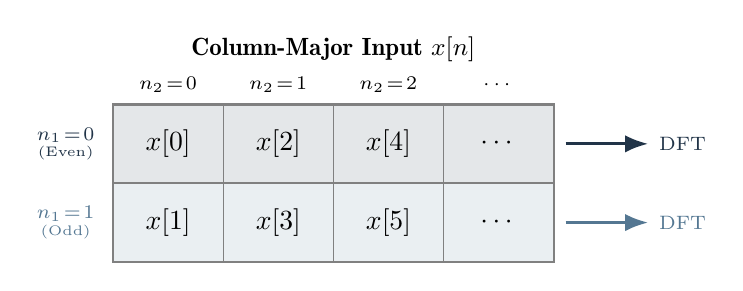
\begin{tikzpicture}[>=Latex, thick]
                    \def\cw{1.4} \def\ch{1.0}
                    % Title
                    \node[font=\small\bfseries] at (2*\cw, 2*\ch+0.7) {Column-Major Input $x[n]$};
                    % Row backgrounds
                    \fill[PrimaryColor!12] (0, \ch) rectangle (4*\cw, 2*\ch);
                    \fill[SecondaryColor!12] (0, 0) rectangle (4*\cw, \ch);
                    % Grid
                    \draw[gray] (0,0) rectangle (4*\cw, 2*\ch);
                    \foreach \i in {1,2,3} {\draw[gray, thin] (\i*\cw, 0) -- (\i*\cw, 2*\ch);}
                    \draw[gray] (0, \ch) -- (4*\cw, \ch);
                    % Column headers
                    \node[font=\scriptsize] at (0.5*\cw, 2*\ch+0.25) {$n_2\!=\!0$};
                    \node[font=\scriptsize] at (1.5*\cw, 2*\ch+0.25) {$n_2\!=\!1$};
                    \node[font=\scriptsize] at (2.5*\cw, 2*\ch+0.25) {$n_2\!=\!2$};
                    \node[font=\scriptsize] at (3.5*\cw, 2*\ch+0.25) {$\cdots$};
                    % Row labels
                    \node[font=\scriptsize, PrimaryColor, align=center] at (-0.6, 1.5*\ch) {$n_1\!=\!0$\\[-2pt]\tiny(Even)};
                    \node[font=\scriptsize, SecondaryColor, align=center] at (-0.6, 0.5*\ch) {$n_1\!=\!1$\\[-2pt]\tiny(Odd)};
                    % Row 0 (even)
                    \node at (0.5*\cw, 1.5*\ch) {$x[0]$};
                    \node at (1.5*\cw, 1.5*\ch) {$x[2]$};
                    \node at (2.5*\cw, 1.5*\ch) {$x[4]$};
                    \node at (3.5*\cw, 1.5*\ch) {$\cdots$};
                    % Row 1 (odd)
                    \node at (0.5*\cw, 0.5*\ch) {$x[1]$};
                    \node at (1.5*\cw, 0.5*\ch) {$x[3]$};
                    \node at (2.5*\cw, 0.5*\ch) {$x[5]$};
                    \node at (3.5*\cw, 0.5*\ch) {$\cdots$};
                    % Row DFT arrows (1st DFT) →
                    \draw[->, PrimaryColor, very thick] (4*\cw+0.15, 1.5*\ch) -- (4*\cw+1.2, 1.5*\ch)
                    node[right, font=\scriptsize] {DFT};
                    \draw[->, SecondaryColor, very thick] (4*\cw+0.15, 0.5*\ch) -- (4*\cw+1.2, 0.5*\ch)
                    node[right, font=\scriptsize] {DFT};
                \end{tikzpicture}
            }

            \vspace{0.5cm}
            \resizebox{\columnwidth}{!}{
                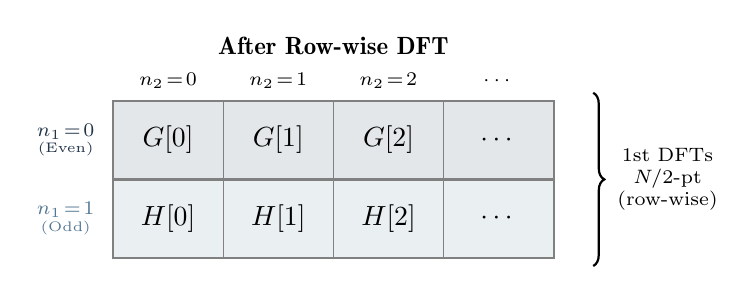
\begin{tikzpicture}[>=Latex, thick]
                    \def\cw{1.4} \def\ch{1.0}
                    % Title
                    \node[font=\small\bfseries] at (2*\cw, 2*\ch+0.7) {After Row-wise DFT};
                    % Row backgrounds
                    \fill[PrimaryColor!12] (0, \ch) rectangle (4*\cw, 2*\ch);
                    \fill[SecondaryColor!12] (0, 0) rectangle (4*\cw, \ch);
                    % Grid
                    \draw[gray] (0,0) rectangle (4*\cw, 2*\ch);
                    \foreach \i in {1,2,3} {\draw[gray, thin] (\i*\cw, 0) -- (\i*\cw, 2*\ch);}
                    \draw[gray] (0, \ch) -- (4*\cw, \ch);
                    % Column headers
                    \node[font=\scriptsize] at (0.5*\cw, 2*\ch+0.25) {$n_2\!=\!0$};
                    \node[font=\scriptsize] at (1.5*\cw, 2*\ch+0.25) {$n_2\!=\!1$};
                    \node[font=\scriptsize] at (2.5*\cw, 2*\ch+0.25) {$n_2\!=\!2$};
                    \node[font=\scriptsize] at (3.5*\cw, 2*\ch+0.25) {$\cdots$};
                    % Row labels
                    \node[font=\scriptsize, PrimaryColor, align=center] at (-0.6, 1.5*\ch) {$n_1\!=\!0$\\[-2pt]\tiny(Even)};
                    \node[font=\scriptsize, SecondaryColor, align=center] at (-0.6, 0.5*\ch) {$n_1\!=\!1$\\[-2pt]\tiny(Odd)};
                    % Row 0 (even)
                    \node at (0.5*\cw, 1.5*\ch) {$G[0]$};
                    \node at (1.5*\cw, 1.5*\ch) {$G[1]$};
                    \node at (2.5*\cw, 1.5*\ch) {$G[2]$};
                    \node at (3.5*\cw, 1.5*\ch) {$\cdots$};
                    % Row 1 (odd)
                    \node at (0.5*\cw, 0.5*\ch) {$H[0]$};
                    \node at (1.5*\cw, 0.5*\ch) {$H[1]$};
                    \node at (2.5*\cw, 0.5*\ch) {$H[2]$};
                    \node at (3.5*\cw, 0.5*\ch) {$\cdots$};
                    % Brace for 1st DFT
                    \draw[decorate, decoration={brace, amplitude=4pt}]
                    (4*\cw+0.5, 2*\ch+0.1) -- (4*\cw+0.5, -0.1)
                    node[midway, right=5pt, font=\scriptsize, align=center] {1st DFTs\\$N/2$-pt\\(row-wise)};
                \end{tikzpicture}
            }
        \end{column}
    \end{columns}
\end{frame}

\begin{frame}{Radix-2 DIT: Twiddle Factors \& Column DFTs}
    \begin{columns}
        \begin{column}{0.55\textwidth}
            \begin{itemize}
                \item After row DFTs, multiply row $n_1$ by twiddle factors $W_N^{n_1 k}$.
                      \begin{itemize}
                          \item Row 0: $\times W_N^0 = 1$
                          \item Row 1: $\times W_N^{k}$
                      \end{itemize}
                \item \textbf{2nd DFT:} Perform 2-point DFT down each column $(\downarrow)$.
                \item This is exactly the butterfly!
                      \begin{align*}
                          X[k]                  & = G[k] + W_N^{k} H[k] \\
                          X[k\!+\!\tfrac{N}{2}] & = G[k] - W_N^{k} H[k]
                      \end{align*}
                \item We obtain the DFT of the original sequence $x[n]$!
                \item Row 0 gives $X[0 \dots N/2\!-\!1]$, \\
                      row 1 gives $X[N/2 \dots N\!-\!1]$.
                \item But the output occurs in \textbf{row-major} order.
            \end{itemize}
        \end{column}
        \begin{column}{0.45\textwidth}
            \centering
            \vspace{0.1cm}
            \resizebox{\columnwidth}{!}{
                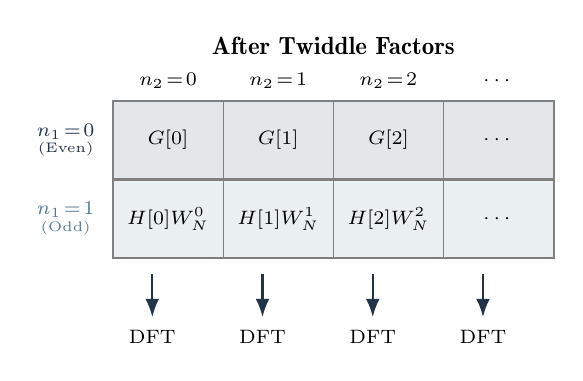
\begin{tikzpicture}[>=Latex, thick]
                    \def\cw{1.4} \def\ch{1.0}
                    % Title
                    \node[font=\small\bfseries] at (2*\cw, 2*\ch+0.7) {After Twiddle Factors};
                    % Row backgrounds
                    \fill[PrimaryColor!12] (0, \ch) rectangle (4*\cw, 2*\ch);
                    \fill[SecondaryColor!12] (0, 0) rectangle (4*\cw, \ch);
                    % Grid
                    \draw[gray] (0,0) rectangle (4*\cw, 2*\ch);
                    \foreach \i in {1,2,3} {\draw[gray, thin] (\i*\cw, 0) -- (\i*\cw, 2*\ch);}
                    \draw[gray] (0, \ch) -- (4*\cw, \ch);
                    % Column headers
                    \node[font=\scriptsize] at (0.5*\cw, 2*\ch+0.25) {$n_2\!=\!0$};
                    \node[font=\scriptsize] at (1.5*\cw, 2*\ch+0.25) {$n_2\!=\!1$};
                    \node[font=\scriptsize] at (2.5*\cw, 2*\ch+0.25) {$n_2\!=\!2$};
                    \node[font=\scriptsize] at (3.5*\cw, 2*\ch+0.25) {$\cdots$};
                    % Row labels
                    \node[font=\scriptsize, PrimaryColor, align=center] at (-0.6, 1.5*\ch) {$n_1\!=\!0$\\[-2pt]\tiny(Even)};
                    \node[font=\scriptsize, SecondaryColor, align=center] at (-0.6, 0.5*\ch) {$n_1\!=\!1$\\[-2pt]\tiny(Odd)};
                    % Row 0 (even)
                    \node[font=\scriptsize] at (0.5*\cw, 1.5*\ch) {$G[0]$};
                    \node[font=\scriptsize] at (1.5*\cw, 1.5*\ch) {$G[1]$};
                    \node[font=\scriptsize] at (2.5*\cw, 1.5*\ch) {$G[2]$};
                    \node[font=\scriptsize] at (3.5*\cw, 1.5*\ch) {$\cdots$};
                    % Row 1 (odd)
                    \node[font=\scriptsize] at (0.5*\cw, 0.5*\ch) {$H[0] W_N^{0}$};
                    \node[font=\scriptsize] at (1.5*\cw, 0.5*\ch) {$H[1] W_N^{1}$};
                    \node[font=\scriptsize] at (2.5*\cw, 0.5*\ch) {$H[2] W_N^{2}$};
                    \node[font=\scriptsize] at (3.5*\cw, 0.5*\ch) {$\cdots$};
                    % Row DFT arrows (1st DFT) →
                    \foreach \k in {0,1,2,3} {
                            \draw[->, PrimaryColor, thick] (\k*\cw+0.5, -0.2) -- (\k*\cw+0.5, -0.75);
                            \node[font=\scriptsize] at (\k*\cw+0.5, -1.0) {DFT};
                        }
                \end{tikzpicture}
            }

            \vspace{0.5cm}
            \resizebox{\columnwidth}{!}{
                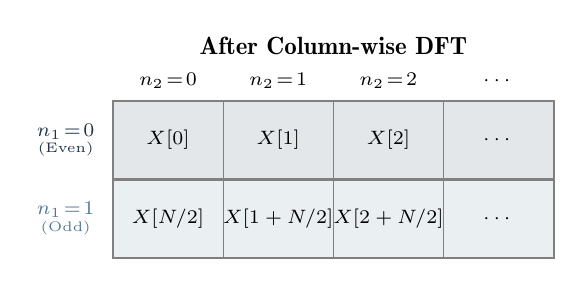
\begin{tikzpicture}[>=Latex, thick]
                    \def\cw{1.4} \def\ch{1.0}
                    % Title
                    \node[font=\small\bfseries] at (2*\cw, 2*\ch+0.7) {After Column-wise DFT};
                    % Row backgrounds
                    \fill[PrimaryColor!12] (0, \ch) rectangle (4*\cw, 2*\ch);
                    \fill[SecondaryColor!12] (0, 0) rectangle (4*\cw, \ch);
                    % Grid
                    \draw[gray] (0,0) rectangle (4*\cw, 2*\ch);
                    \foreach \i in {1,2,3} {\draw[gray, thin] (\i*\cw, 0) -- (\i*\cw, 2*\ch);}
                    \draw[gray] (0, \ch) -- (4*\cw, \ch);
                    % Column headers
                    \node[font=\scriptsize] at (0.5*\cw, 2*\ch+0.25) {$n_2\!=\!0$};
                    \node[font=\scriptsize] at (1.5*\cw, 2*\ch+0.25) {$n_2\!=\!1$};
                    \node[font=\scriptsize] at (2.5*\cw, 2*\ch+0.25) {$n_2\!=\!2$};
                    \node[font=\scriptsize] at (3.5*\cw, 2*\ch+0.25) {$\cdots$};
                    % Row labels
                    \node[font=\scriptsize, PrimaryColor, align=center] at (-0.6, 1.5*\ch) {$n_1\!=\!0$\\[-2pt]\tiny(Even)};
                    \node[font=\scriptsize, SecondaryColor, align=center] at (-0.6, 0.5*\ch) {$n_1\!=\!1$\\[-2pt]\tiny(Odd)};
                    % Row 0 (even)
                    \node[font=\scriptsize] at (0.5*\cw, 1.5*\ch) {$X[0]$};
                    \node[font=\scriptsize] at (1.5*\cw, 1.5*\ch) {$X[1]$};
                    \node[font=\scriptsize] at (2.5*\cw, 1.5*\ch) {$X[2]$};
                    \node[font=\scriptsize] at (3.5*\cw, 1.5*\ch) {$\cdots$};
                    % Row 1 (odd)
                    \node[font=\scriptsize] at (0.5*\cw, 0.5*\ch) {$X[N/2]$};
                    \node[font=\scriptsize] at (1.5*\cw, 0.5*\ch) {$X[1+N/2]$};
                    \node[font=\scriptsize] at (2.5*\cw, 0.5*\ch) {$X[2+N/2]$};
                    \node[font=\scriptsize] at (3.5*\cw, 0.5*\ch) {$\cdots$};
                \end{tikzpicture}
            }
        \end{column}
    \end{columns}
\end{frame}

\begin{frame}{Radix-2 DIT: Twiddle Factors \& Column DFTs}
    \begin{columns}
        \begin{column}{0.55\textwidth}
            \begin{itemize}
                \item We want $X[k]$ in the correct order. We want the transpose matrix.
                \item Mathematically, for
                      \begin{align*}
                          k_1 & = \text{row index} \in \{0, 1\}                 \\
                          k_2 & = \text{column index} \in \{0, \dots, N/2-1\} &
                      \end{align*}
                \item We want the \textbf{row-major} indexing:
                      \begin{align*}
                          k = (N/2) k_1 + k_2
                      \end{align*}
                \item Using this index, we can write:
                      \begin{align*}
                          X[(N/2)k_1 + k_2] = G[k_2] + W^{k_1}_2 \left(W_N^{k_2} H[k_2]\right)
                      \end{align*}
                \item Not the final form yet!
                \item But \textbf{key take away}:
                      We can visualize Cooley-Tukey algorithm as arranging numbers on a matrix, performing DFTs on columns and rows!

            \end{itemize}
        \end{column}
        \begin{column}{0.45\textwidth}
            \centering
            \vspace{0.1cm}
            \resizebox{\columnwidth}{!}{
                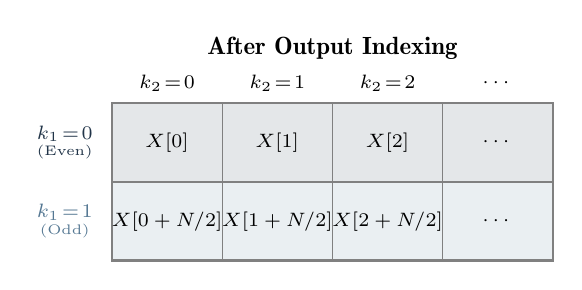
\begin{tikzpicture}[>=Latex, thick]
                    \def\cw{1.4} \def\ch{1.0}
                    % Title
                    \node[font=\small\bfseries] at (2*\cw, 2*\ch+0.7) {After Output Indexing};
                    % Row backgrounds
                    \fill[PrimaryColor!12] (0, \ch) rectangle (4*\cw, 2*\ch);
                    \fill[SecondaryColor!12] (0, 0) rectangle (4*\cw, \ch);
                    % Grid
                    \draw[gray] (0,0) rectangle (4*\cw, 2*\ch);
                    \foreach \i in {1,2,3} {\draw[gray, thin] (\i*\cw, 0) -- (\i*\cw, 2*\ch);}
                    \draw[gray] (0, \ch) -- (4*\cw, \ch);
                    % Column headers
                    \node[font=\scriptsize] at (0.5*\cw, 2*\ch+0.25) {$k_2\!=\!0$};
                    \node[font=\scriptsize] at (1.5*\cw, 2*\ch+0.25) {$k_2\!=\!1$};
                    \node[font=\scriptsize] at (2.5*\cw, 2*\ch+0.25) {$k_2\!=\!2$};
                    \node[font=\scriptsize] at (3.5*\cw, 2*\ch+0.25) {$\cdots$};
                    % Row labels
                    \node[font=\scriptsize, PrimaryColor, align=center] at (-0.6, 1.5*\ch) {$k_1\!=\!0$\\[-2pt]\tiny(Even)};
                    \node[font=\scriptsize, SecondaryColor, align=center] at (-0.6, 0.5*\ch) {$k_1\!=\!1$\\[-2pt]\tiny(Odd)};
                    % Row 0 (even)
                    \node[font=\scriptsize] at (0.5*\cw, 1.5*\ch) {$X[0]$};
                    \node[font=\scriptsize] at (1.5*\cw, 1.5*\ch) {$X[1]$};
                    \node[font=\scriptsize] at (2.5*\cw, 1.5*\ch) {$X[2]$};
                    \node[font=\scriptsize] at (3.5*\cw, 1.5*\ch) {$\cdots$};
                    % Row 1 (odd)
                    \node[font=\scriptsize] at (0.5*\cw, 0.5*\ch) {$X[0+N/2]$};
                    \node[font=\scriptsize] at (1.5*\cw, 0.5*\ch) {$X[1+N/2]$};
                    \node[font=\scriptsize] at (2.5*\cw, 0.5*\ch) {$X[2+N/2]$};
                    \node[font=\scriptsize] at (3.5*\cw, 0.5*\ch) {$\cdots$};

                \end{tikzpicture}
            }
        \end{column}
    \end{columns}
\end{frame}


\begin{frame}{Radix-3 DIT DFT: Derivation}
    \begin{itemize}
        \item The same idea extends naturally. For $N = 3 N_2$, split $x[n]$ into three subsequences by index modulo 3:
              \begin{align*}
                  X[k] & = \sum_{r=0}^{N/3-1} x[3r]\, W_{N/3}^{rk} + W_N^k \sum_{r=0}^{N/3-1} x[3r+1]\, W_{N/3}^{rk} + W_N^{2k} \sum_{r=0}^{N/3-1} x[3r+2]\, W_{N/3}^{rk}
              \end{align*}
        \item Define three $N/3$-point DFTs:
              \begin{equation*}
                  G_m[k] = \sum_{r=0}^{N/3-1} x[3r+m]\, W_{N/3}^{rk} \qquad m \in \{0, 1, 2\}
              \end{equation*}
    \end{itemize}
    \begin{conceptbox}{Radix-3 DIT Combination}
        \begin{align*}
            X[k] = G_0[k] + (W_N^{k}\, G_1[k]) + (W_N^{2k}\, G_2[k])                   \\
            X[k+N/3] = G_0[k] + W_3^{1}(W_N^{k}\, G_1[k]) + W_3^{2}(W_N^{2k}\, G_2[k]) \\
            X[k+2N/3] = G_0[k] + W_3^{2}(W_N^{k}\, G_1[k]) + W_3^{4}(W_N^{2k}\, G_2[k])
        \end{align*}
    \end{conceptbox}
    \begin{itemize}
        \item The above 3 equations are also a 3-point DFT!
    \end{itemize}
\end{frame}

\begin{frame}{Radix-3 DIT: Tabular Interpretation ($N_1=3, N_2=N/3$)}
    \begin{columns}[T]
        \begin{column}{0.40\textwidth}
            \begin{itemize}
                \item Load $x[n]$ into a $3 \times N/3$ matrix, \textbf{column-major}: $n = 3n_2 + n_1$.
                \item \textcolor{PrimaryColor}{\textbf{Row 0}}: $n \equiv 0 \pmod{3}$
                \item \textcolor{SecondaryColor}{\textbf{Row 1}}: $n \equiv 1 \pmod{3}$
                \item \textcolor{AccentColor}{\textbf{Row 2}}: $n \equiv 2 \pmod{3}$
            \end{itemize}
            \vspace{0.15cm}
            \begin{enumerate}
                \item \textbf{1st DFTs:} $N/3$-point DFT along each row $(\rightarrow)$.
                \item Multiply by twiddle $W_N^{n_1 k_2}$.
                \item \textbf{2nd DFTs:} 3-point DFT down each column $(\downarrow)$.
            \end{enumerate}
            \vspace{0.15cm}
            \begin{itemize}
                \item Take output \textbf{row-major}: $k = (N/3)\,k_1 + k_2$.
            \end{itemize}
        \end{column}
        \begin{column}{0.57\textwidth}
            \centering
            \vspace{0.1cm}
            \resizebox{\columnwidth}{!}{
                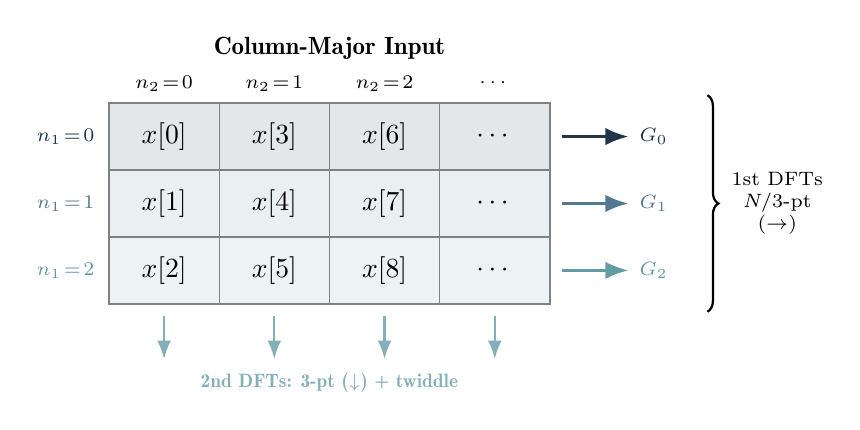
\begin{tikzpicture}[>=Latex, thick]
                    \def\cw{1.4} \def\ch{0.85}
                    % Title
                    \node[font=\small\bfseries] at (2*\cw, 3*\ch+0.7) {Column-Major Input};
                    % Row backgrounds (3 rows)
                    \fill[PrimaryColor!12] (0, 2*\ch) rectangle (4*\cw, 3*\ch);
                    \fill[SecondaryColor!12] (0, \ch) rectangle (4*\cw, 2*\ch);
                    \fill[AccentColor!12] (0, 0) rectangle (4*\cw, \ch);
                    % Grid
                    \draw[gray] (0,0) rectangle (4*\cw, 3*\ch);
                    \foreach \i in {1,2,3} {\draw[gray, thin] (\i*\cw, 0) -- (\i*\cw, 3*\ch);}
                    \draw[gray] (0, \ch) -- (4*\cw, \ch);
                    \draw[gray] (0, 2*\ch) -- (4*\cw, 2*\ch);
                    % Column headers
                    \node[font=\scriptsize] at (0.5*\cw, 3*\ch+0.25) {$n_2\!=\!0$};
                    \node[font=\scriptsize] at (1.5*\cw, 3*\ch+0.25) {$n_2\!=\!1$};
                    \node[font=\scriptsize] at (2.5*\cw, 3*\ch+0.25) {$n_2\!=\!2$};
                    \node[font=\scriptsize] at (3.5*\cw, 3*\ch+0.25) {$\cdots$};
                    % Row labels
                    \node[font=\scriptsize, PrimaryColor, align=center] at (-0.55, 2.5*\ch) {$n_1\!=\!0$};
                    \node[font=\scriptsize, SecondaryColor, align=center] at (-0.55, 1.5*\ch) {$n_1\!=\!1$};
                    \node[font=\scriptsize, AccentColor, align=center] at (-0.55, 0.5*\ch) {$n_1\!=\!2$};
                    % Row 0
                    \node at (0.5*\cw, 2.5*\ch) {$x[0]$};
                    \node at (1.5*\cw, 2.5*\ch) {$x[3]$};
                    \node at (2.5*\cw, 2.5*\ch) {$x[6]$};
                    \node at (3.5*\cw, 2.5*\ch) {$\cdots$};
                    % Row 1
                    \node at (0.5*\cw, 1.5*\ch) {$x[1]$};
                    \node at (1.5*\cw, 1.5*\ch) {$x[4]$};
                    \node at (2.5*\cw, 1.5*\ch) {$x[7]$};
                    \node at (3.5*\cw, 1.5*\ch) {$\cdots$};
                    % Row 2
                    \node at (0.5*\cw, 0.5*\ch) {$x[2]$};
                    \node at (1.5*\cw, 0.5*\ch) {$x[5]$};
                    \node at (2.5*\cw, 0.5*\ch) {$x[8]$};
                    \node at (3.5*\cw, 0.5*\ch) {$\cdots$};
                    % Row DFT arrows (1st DFT) →
                    \draw[->, PrimaryColor, very thick] (4*\cw+0.15, 2.5*\ch) -- (4*\cw+1.0, 2.5*\ch)
                    node[right, font=\scriptsize] {$G_0$};
                    \draw[->, SecondaryColor, very thick] (4*\cw+0.15, 1.5*\ch) -- (4*\cw+1.0, 1.5*\ch)
                    node[right, font=\scriptsize] {$G_1$};
                    \draw[->, AccentColor, very thick] (4*\cw+0.15, 0.5*\ch) -- (4*\cw+1.0, 0.5*\ch)
                    node[right, font=\scriptsize] {$G_2$};
                    % Brace
                    \draw[decorate, decoration={brace, amplitude=4pt}]
                    (4*\cw+2.0, 3*\ch+0.1) -- (4*\cw+2.0, -0.1)
                    node[midway, right=5pt, font=\scriptsize, align=center] {1st DFTs\\$N/3$-pt\\($\rightarrow$)};
                    % Column DFT arrows (2nd DFT) ↓
                    \foreach \i in {0,1,2,3} {
                            \draw[->, AccentColor!80, thick] (\i*\cw+0.5*\cw, -0.15) -- (\i*\cw+0.5*\cw, -0.7);
                        }
                    \node[font=\scriptsize\bfseries, AccentColor!80] at (2*\cw, -1.0) {2nd DFTs: 3-pt ($\downarrow$) + twiddle};
                \end{tikzpicture}
            }
        \end{column}
    \end{columns}
\end{frame}

\begin{frame}{General Cooley-Tukey Factorization ($N = N_1 N_2$)}
    \begin{itemize}
        \item Having seen the tabular view for Radix-2 and Radix-3, let's formalize the general $N_1 \times N_2$ factorization.
        \item Re-index the input $n$ as an $N_1 \times N_2$ matrix in \textbf{column-major order}:
              \begin{equation*}
                  n = N_1 n_2 + n_1 \qquad \begin{cases} n_1 \in \{0, 1, \dots, N_1-1\} \\ n_2 \in \{0, 1, \dots, N_2-1\} \end{cases}
              \end{equation*}
              Substituting this into the DFT definition yields a 2D sum:
              \begin{equation*}
                  X[k] = \sum_{n_1=0}^{N_1-1} \sum_{n_2=0}^{N_2-1} x[{N_1 n_2 + n_1}] e^{-\frac{2\pi i}{N} (N_1 n_2 + n_1)k}
              \end{equation*}
        \item Re-index the output $k$ as an $N_1 \times N_2$ matrix in \textbf{row-major order}:
              \begin{equation*}
                  k = N_2 k_1 + k_2 \qquad \begin{cases} k_1 \in \{0, 1, \dots, N_1-1\} \\ k_2 \in \{0, 1, \dots, N_2-1\} \end{cases}
              \end{equation*}
    \end{itemize}
\end{frame}

\begin{frame}{General Cooley-Tukey Factorization ($N = N_1 N_2$)}
    \begin{itemize}
        \item Substitute $k = N_2 k_1 + k_2$ into the exponent $(N_1 n_2 + n_1)k$:
              \begin{align*}
                  (N_1 n_2 + n_1)(N_2 k_1 + k_2) & = N_1 N_2 n_2 k_1 + N_1 n_2 k_2 + N_2 n_1 k_1 + n_1 k_2 \\
                                                 & = N n_2 k_1 + N_1 n_2 k_2 + N_2 n_1 k_1 + n_1 k_2
              \end{align*}
        \item The first term's exponential is $e^{-\frac{2\pi i}{N} N n_2 k_1} = 1$, so this cross term vanishes.
        \item We separate the remaining terms in the exponential $e^{-\frac{2\pi i}{N}(\dots)}$:
              \begin{equation*}
                  e^{-\frac{2\pi i}{N_2} n_2 k_2} \cdot e^{-\frac{2\pi i}{N_1} n_1 k_1} \cdot e^{-\frac{2\pi i}{N} n_1 k_2}
              \end{equation*}
        \item Substituting this back into the double sum and rearranging:
    \end{itemize}
\end{frame}

\begin{frame}{General Cooley-Tukey Factorization ($N = N_1 N_2$)}
    \begin{conceptbox}{Cooley-Tukey 2D Matrix Formulation}
        \begin{equation*}
            X[{N_2 k_1 + k_2}] = \sum_{n_1=0}^{N_1-1} \underbrace{\left[ e^{-\frac{2\pi i}{N_1 N_2} n_1 k_2} \right]}_{\text{Twiddle Factor}} \left( \sum_{n_2=0}^{N_2-1} x[{N_1 n_2 + n_1}] e^{-\frac{2\pi i}{N_2} n_2 k_2} \right) e^{-\frac{2\pi i}{N_1} n_1 k_1}
        \end{equation*}
    \end{conceptbox}
    \vspace{0.2cm}
    \begin{itemize}
        \item \textbf{Inner Sum:} An $N_2$-point DFT on the rows of the $N_1 \times N_2$ input matrix.
        \item \textbf{Twiddle Factors:} The bracketed term scales the intermediate results by $e^{-\frac{2\pi i}{N_1 N_2} n_1 k_2}$.
        \item \textbf{Outer Sum:} An $N_1$-point DFT down the columns of the intermediate matrix.
    \end{itemize}
\end{frame}

\begin{frame}{Bailey's FFT Algorithm}
    \begin{itemize}
        \item The Cooley-Tukey matrix formulation directly yields \textbf{Bailey's FFT} (a.k.a.\ the Four-Step FFT):
    \end{itemize}
    \vspace{0.1cm}
    \begin{algorithmbox}{Bailey's FFT}
        \begin{enumerate}
            \item Arrange input $x[n]$ in an $N_1 \times N_2$ matrix (column-major).
            \item Compute $N_2$-point DFT of each row $(\rightarrow)$.
            \item Multiply entry $(n_1, k_2)$ by twiddle factor $W_N^{n_1 k_2}$.
            \item Compute $N_1$-point DFT of each column $(\downarrow)$.
        \end{enumerate}
    \end{algorithmbox}
    \vspace{0.2cm}
    \begin{itemize}
        \item How to compute the $N_1$- and $N_2$-point DFTs? \textbf{Apply the same algorithm recursively!}
        \item If $N = p_1^{a_1} p_2^{a_2} \cdots$, we recursively factor until only small primes remain $\Rightarrow$ $O(N \log N)$ for any composite $N$.
        \item This handles powers of 2, powers of 3, mixed radices—any $N$ with small prime factors.
        \item But what if $N$ itself is a \textbf{large prime}?
    \end{itemize}
\end{frame}

\end{document}
